\subsection{Функциональная модель программного средства}
\label{sec:domain:model}

Функциональная модель программного средства представлена в виде диаграммы вариантов использования и информационной
модели предметной области. Варианты использования отражают функциональность системы в ответ на внешние воздействия с
точки зрения получения значимого результата для пользователей. Информационная модель предметной области в
дальнейшем будет использоваться при проектировании базы данных для программного средства.

\subsubsection{} Варианты использования программного средства
\label{sec:domain:model:use_cases}

Проектируемое программное средство предполагает, что пользователи делятся на обычных и менеджеров.

Возможности обычного пользователя и менеджера представлены на рисунке \ref{fig:domain:model:use_cases} в виде
диаграммы вариантов использования, разработанной с использованием нотации UML 2.1.

Рассмотрим подробно представленные на рисунке прецеденты.

Регистрация, аутентификация и авторизация – функции, которые доступны для роли «Гость» (пользователь, не
зарегистрированный в системе). В первой версии приложения планируется реализация собственной системы авторизации; в
дальнейшем будет добавлена возможность регистрации с помощью внешних поставщиков данных (Google).

После регистрации пользователь получает доступ к фунциям заполнения профиля. Среди функций заполнения профиля стоит
отметить:

\begin{sidewaysfigure}
  \centering
    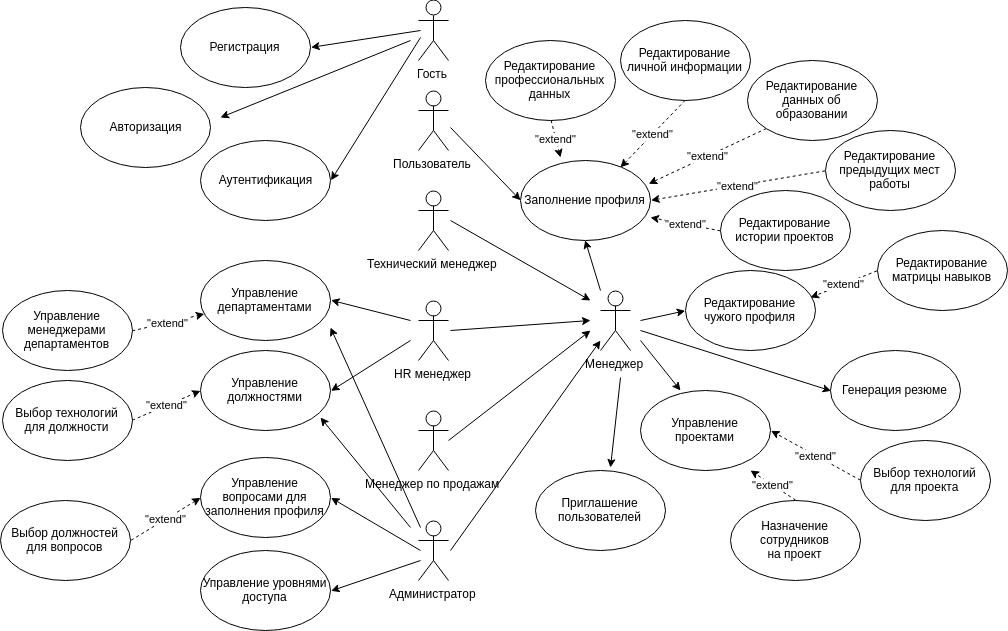
\includegraphics[scale=0.7]{use_case.png} 
    \caption{Диаграмма вариантов использования ПС}
    \label{fig:domain:model:use_cases}
\end{sidewaysfigure}

\begin{itemize}
	\item редактирование личной информации. В эту функцию входит возможность заполнения имени, фамилии, даты рождения,
	адреса электронной почты, места жительства, номера телефона;
  \item редактиование данных об образовании. В этот блок входит возможность ввода учебного заведения или назавния курсов,
  годов начала и конца обучения, возможность указания специализации и ученой степени. Есть возможность добавления
  нескольких мест учебы. Также пользователю предлагается указать свой уровень владения английским языком, что
  является крайне важным фактором при работа в сфере информационных технологий;
	\item редактирование профессиональных данных. В этой секции пользователю предлагается ответить на несколько вопросов,
  связанных с его профессией. Например, разработчику серверной части программного обеспечения будут заданы следующие
  вопросы: "В каких технологиях серверной части ПО вы хороши?", "В каких технологиях клиентской части ПО вы хороши?",
  "С какими базами данных вы имели опыт работы?", "Какие системы управления проектами вы использовали?",
  "С какими методологиями разработки ПО вы знакомы?", "Какие другие инструменты вы использовали в вашей работе?";
	\item редактирование предыдущих мест работы. Здесь можно добавлять предудущие места работы с указанием начала и
  окончания работы. Также есть возможность добавить в свое резюме предудщие рабочие проекты. Здесь можно указать название
  проекта, краткое его описание, зону ответственности, время начала и окончания работы над проектом, роль в команде, 
  а также выбрать из списка технологии, использовавшиеся на данном проекте;
	\item редактирование истории проектов в текущей организации.
\end{itemize}

Кроме обычных пользователей, в системе присутствуют менеджеры, которые обладают этим же функционалом. Кроме того,
все менеджеры имеют следующий набор функций:
\begin{itemize}
	\item Менеджеры имеют возможность редактировать профили других пользователей. Кроме того, они могут редактировать
  матрицу навыков пользователя, чего не может делать обычный пользователь;
  \item менеджеры могут генерировать из заполненого профиля резюме для последующей отправки заказчику;
  \item менеджеры могут управлять проектами в компании. Среди функций управления проектами стоит отметить возможность
  выбора технологий, которые будут использоваться на проекте и возможность назначения сотрудников на проект. Таким образом
  осуществляется отслеживание занятости персонала на проектах;
  \item Менеджер может приглашать в систему новых пользователей посредством отправки писем на указанную электронную
  почту. Условием приглашения пользователя является наличие электронной почты в корпоративном домене.
\end{itemize}

В системе представлены следующие типы менеджеров:

\begin{itemize}
	\item технический менеджер;
	\item HR менеджер;
	\item менеджер по продажам.
\end{itemize}

Технический менеджер и менеджер по продажам имеют возможности обычного менеджера, которые описаны выше, HR менеджер,
кроме вышеперечисленных функиций также имеет возможность управления департаментами в компании(создание, редактирование,
удаление), с возможностью назначения менеджеров(каждый департамент должен иметь своего HR менеджера, технического
менеджера и менеджера по продажам). HR менеджер также имеет доступ к управлению должностями компании с определением
списка технологий, о знании которых может указывать работник при заполнении своего профиля.

Кроме менеджеров, гостей и обычных пользователей, в системе существует еще один вид пользователя -- администратор. 
Помимо всех функций обычного пользователя и менеджеров, администратор также имеет возможность управлять списком
вопросов для каждой должности, которые будут в дальнейшем задаваться при заполнении профессиональных данных пользователя,
и управлять уровнями доступа для менеджеров(можно разрешать или запрещать те или иные действия определенному типу
менеджеров).

\subsubsection{} Разработка инфологической модели базы данных
\label{sec:domain:model:database}

Исходя из необходимости использования в проектируемом приложении базы данных, разработаем ее инфологическую модель.
Для ее создания будем использовать расширение диаграммы классов UML 2.1, предназначенное для моделирования баз данных.
Полученная диаграмма (рисунок~\ref{fig:domain:model:db:model}) будет являться моделью базы данных инфологического
уровня ~\cite{kulikov_db_workbook}.

\begin{figure}[!ht]
	\centering
	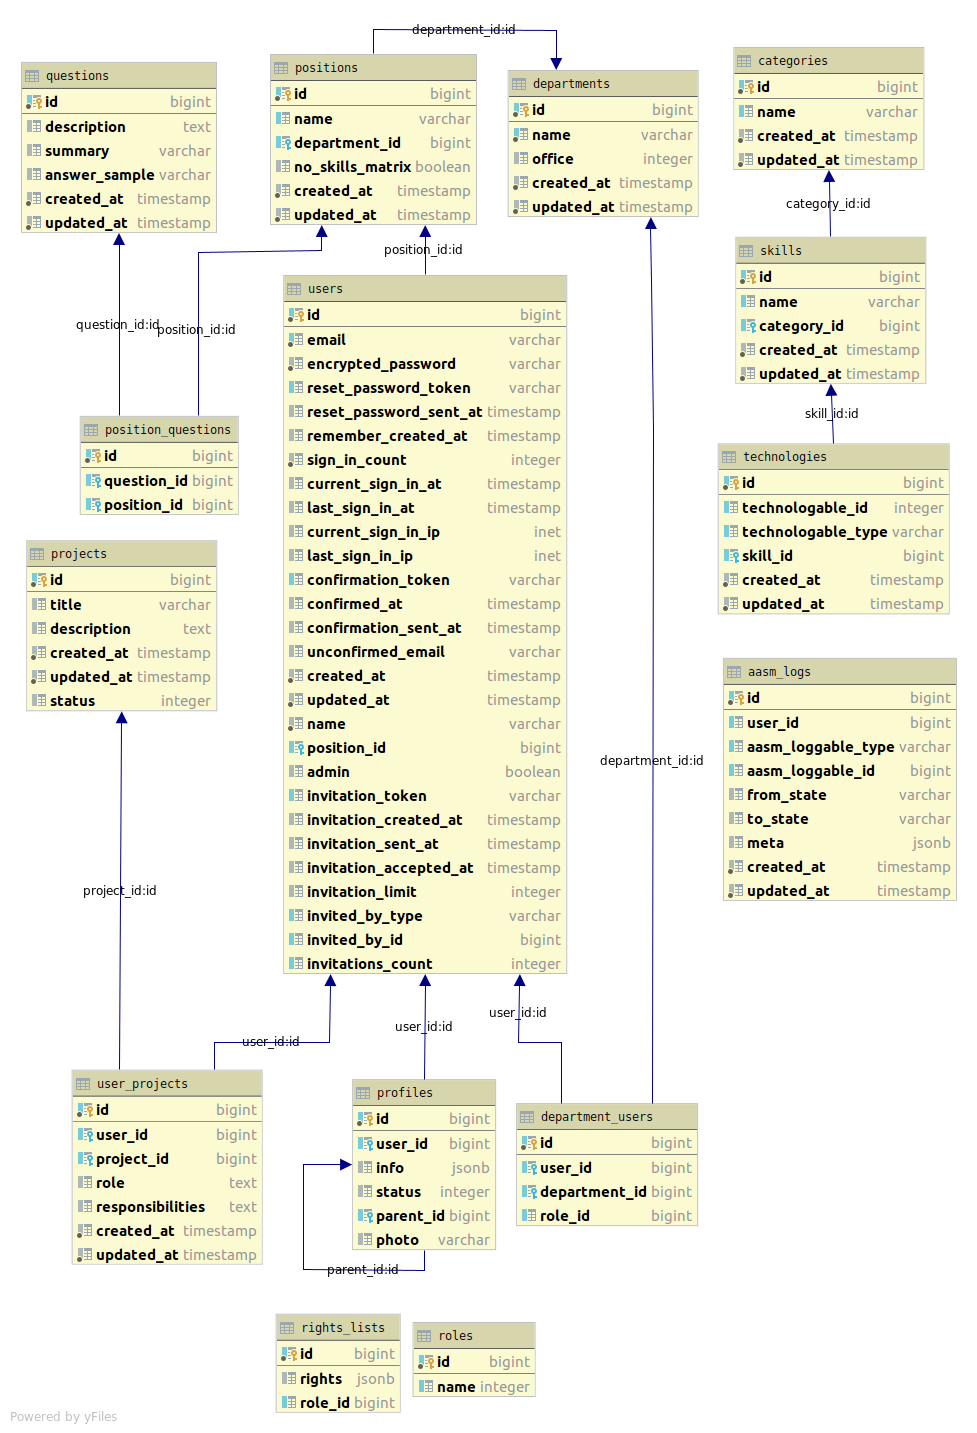
\includegraphics[scale=0.47]{database.png} 
	\caption{Инфологическая модель базы данных}
	\label{fig:domain:model:db:model}
\end{figure}

Предметная область разрабатываемого проекта включает следующие сущности и атрибуты:

\begin{enumerate}
  \item пользователь:
    \begin{enumerate}
      \item адрес электронной почты;
      \item хешированный пароль;
      \item количество авторизаций;
      \item время текущей авторизации;
      \item время последней авторизации;
      \item имя;
      \item идентификатор позиции;
    \end{enumerate}
  \item вопрос:
    \begin{enumerate}
      \item название;
      \item описание;
      \item краткий ответ;
    \end{enumerate}
  \item позиция:
    \begin{enumerate}
      \item название;
      \item идентификатор департамента;
      \item наличие матрицы навыков;
    \end{enumerate}
  \item департамент:
    \begin{enumerate}
      \item название;
      \item офис;
    \end{enumerate}
  \item категория:
    \begin{enumerate}
      \item название;
    \end{enumerate}
  \item навык:
    \begin{enumerate}
      \item название;
      \item идентификатор категории;
    \end{enumerate}
  \item технология:
    \begin{enumerate}
      \item идентификатор технологии;
      \item тип технологии;
      \item идентификатор навыка;
    \end{enumerate}
  \item список прав:
    \begin{enumerate}
      \item права;
      \item идентификатор роли;
    \end{enumerate}
  \item журнал:
    \begin{enumerate}
      \item идентификатор пользователя;
      \item тип журнала;
      \item идентификатор журнала;
      \item исходное состояние;
      \item конечное состояние;
      \item данные;
    \end{enumerate}
  \item роль:
    \begin{enumerate}
      \item название;
    \end{enumerate}
  \item пользователь департамента:
    \begin{enumerate}
      \item идентификатор пользователя;
      \item идентификатор департамента;
      \item идентификатор роли;
    \end{enumerate}
  \item профиль:
    \begin{enumerate}
      \item идентификатор пользователя;
      \item информация;
      \item статус;
      \item идентификатор родителя;
      \item ссылка на фотографию;
    \end{enumerate}
  \item пользователь проекта:
    \begin{enumerate}
      \item идентификатор пользователя;
      \item идентификатор проекта;
      \item роль;
      \item зона ответственности;
    \end{enumerate}
  \item проект:
    \begin{enumerate}
      \item название;
      \item описание;
      \item статус;
    \end{enumerate}
  \pagebreak
  \item вопрос позиции:
    \begin{enumerate}
      \item идентификатор вопроса;
      \item идентификатор позиции.
    \end{enumerate}
\end{enumerate}
